\documentclass[10pt]{article}

\usepackage[table,xcdraw]{xcolor}
\usepackage{graphicx}
\usepackage[left=2.54cm, right=2.54cm, top=3.18cm, bottom=2.54cm]{geometry}
%\usepackage{fontspec}
\usepackage{titlesec}
\usepackage{setspace}
\usepackage{enumitem}
\usepackage{colortbl}
\usepackage{tabularx}
\usepackage{geometry}
\usepackage{float}
\usepackage{fancyhdr}
\pagestyle{fancy}
%\defaultfontfeatures{Mapping=tex-text,Scale=MatchLowercase}
%\setmainfont{Arial}

\definecolor{azure}{RGB}{25,60,102}
\definecolor{darkazure}{RGB}{37,95,166}
\definecolor{danube}{RGB}{106,157,212}


\titleformat{\section}
{\large\bfseries\color{darkazure}}
{}{0.0001em}{}
\renewcommand{\headrulewidth}{0pt}

\rhead{
	\vspace*{-3em}
	
\includegraphics[height=1.45cm]{../assets/mef_logo.png}
}


\begin{document}
	\arrayrulecolor{danube}
	

	
	\begin{spacing}{1.1}
	{\color{azure}
		\bfseries
		\huge{
			\noindent
			COMP492 SENIOR DESIGN PROJECT II \hspace{0pt} \\
			PROPOSAL FORM \par
		}
		\large{
			\noindent
			DEPARTMENT OF COMPUTER ENGINEERING \newline \par
		}
	}
	\end{spacing}
	\vspace{-2em}
	\section{Project Name}
	
	Turkish Question Generation Model
	

	\section{Project Summary (Abstract)}
	
	Question Generation is a Deep Learning model that given a paragraph, passage or an entity in Turkish, produces the possible questions that can be answered solely by the given content to the system. Question Generation(QG) Systems are capable of generating various logical questions from the given text input. QG Systems are prevalent in several computer applications such as chatbots, automated grading systems etc.\newline \par
	
	In this project, our aim is to train different deep learning models for question generation and assess their performances. We find this task worth tackling since there are not many examples of comprehensive studies on the topic and the outcomes of this project will empower the development of more capable-than-ever Question Answering Systems for the Turkish Language. \newline \par
	
	QG models require extensively large training data, thus, in the last semester we have developed the initial dataset for the development of the QG model. This dataset is the largest Turkish Question Answer dataset currently available. In this semester, we also aim to improve the diversity of our dataset to generate questions in larger extent. \newline \par
	
	
	\section{Keywords}
	Natural Language Processing, Deep Learning, Question Generation \newline \par
	
	\section{Hardware and Software Requirements}
	
	\begin{itemize}[label=\textcolor{darkazure}{\Large\textbullet}]
		\item GPU Optimized Server. Will be used for training deep learning models, storing large amounts of data and as a collaborative environment.
		
		\item UNIX Based Environment(s). Given the design and integration of de-facto programming languages, frameworks, tools with Unix based operating systems, along with the flexibility and low-level tools it has to offer, we concluded that UNIX based operating systems will be most suitable for the development process.
		
		\item Dataset.  Contains Turkish paragraphs, related questions and their answers.
	\end{itemize}
	
	
	\section{Project Tasks, Time Plan and Deliverables}
	\begin{center}
		\begin{table}[H]
			\caption{Project tasks, time plan and deliverables}
			\begin{tabularx}{\textwidth}{|>{\raggedright\arraybackslash}m{28mm}|m{20mm}|m{28mm}|m{28mm}|m{39mm}|}					
				\rowcolor[RGB]{215,229,244}
				\hline
				\multicolumn{1}{|>{\centering\arraybackslash}m{28mm}|}{\textbf{Task}} 
				& \multicolumn{1}{>{\centering\arraybackslash}m{20mm}|}{\textbf{Start \& Due \newline Dates}} 
				& \multicolumn{1}{>{\centering\arraybackslash}m{28mm}|}{\textbf{Deliverable}} 
				& \multicolumn{1}{>{\centering\arraybackslash}m{28mm}|}{\textbf{Evaluation Criteria}} 
				& \multicolumn{1}{>{\centering\arraybackslash}m{39mm}|}{\textbf{Objective}}\\
				Project Proposal & 22/02/2021\newline 05/03/2021 & Proposal with clear goals. & Readable, clear & Expressing our intent for the research project and our tasks for this semester. \\ \hline
				
				Literature Review and data collection & 01/03/2021\newline12/03/2021 & A collection of related papers and a training dataset for QG. & Moderate size dataset and collection of recent publications & Learning the foundations of the learning-based methods, developing insight about the concepts. Learning state-of-the art in this research area. Collecting the first Turkish QG dataset. \\ \hline  
				
				Development\newline Environment\newline Preparation & 04/03/2021\newline10/03/2021 & A working environment & Installment of necessary tools, programming languages etc. & Embracing the concepts of the operating system, programming language, frameworks and best practices to be used during the development stages \\ \hline  
				
				Revision of the dataset from COMP491 & 08/01/2021\newline12/03/2021 & Revision of the the dataset & Completeness & Covering and revising the work done in detail from COMP491. \\ \hline  
				
				Technical Preparation & 12/03/2021\newline 25/03/2021 & N/A. & N/A. & Preparing the basis for our further work. \\ \hline
				
				Implementation of Models & 19/03/2021\newline 15/04/2021 & Working prototypes. & Accuracy, performance, capable models & Generating questions in different forms from a given text by using trained models. \\ \hline
				
				Progress Report \& Presentation Preparation & 06/04/2021\newline 09/04/2021 & Well-prepared report and presentation. & Complete, readable, formatted & Covering the work done in detail up to middle of the semester. \\ \hline
				
				Evaluation of Models & 19/04/2021\newline 30/04/2021 & Report for evaluation of models  & Comprehensive, readable, clear & Evaluating the trained models with the state-of-art QG evaluation metrics \\ \hline
				
				User Interface Development & 03/05/2021\newline 21/05/2021 & Simple UI for users to interact & Simple to use, error-free usage & Enabling the users to interact with the QG model  \\ \hline
				
				Final Report \& Presentation Preparation & 20/05/2021\newline 02/06/2021 & Well-prepared report and presentation & Complete, readable, formatted & Covering the work done in detail. \\ \hline
			\end{tabularx}
		\end{table}
	\end{center}
	\begin{figure}[H]
		\centering
		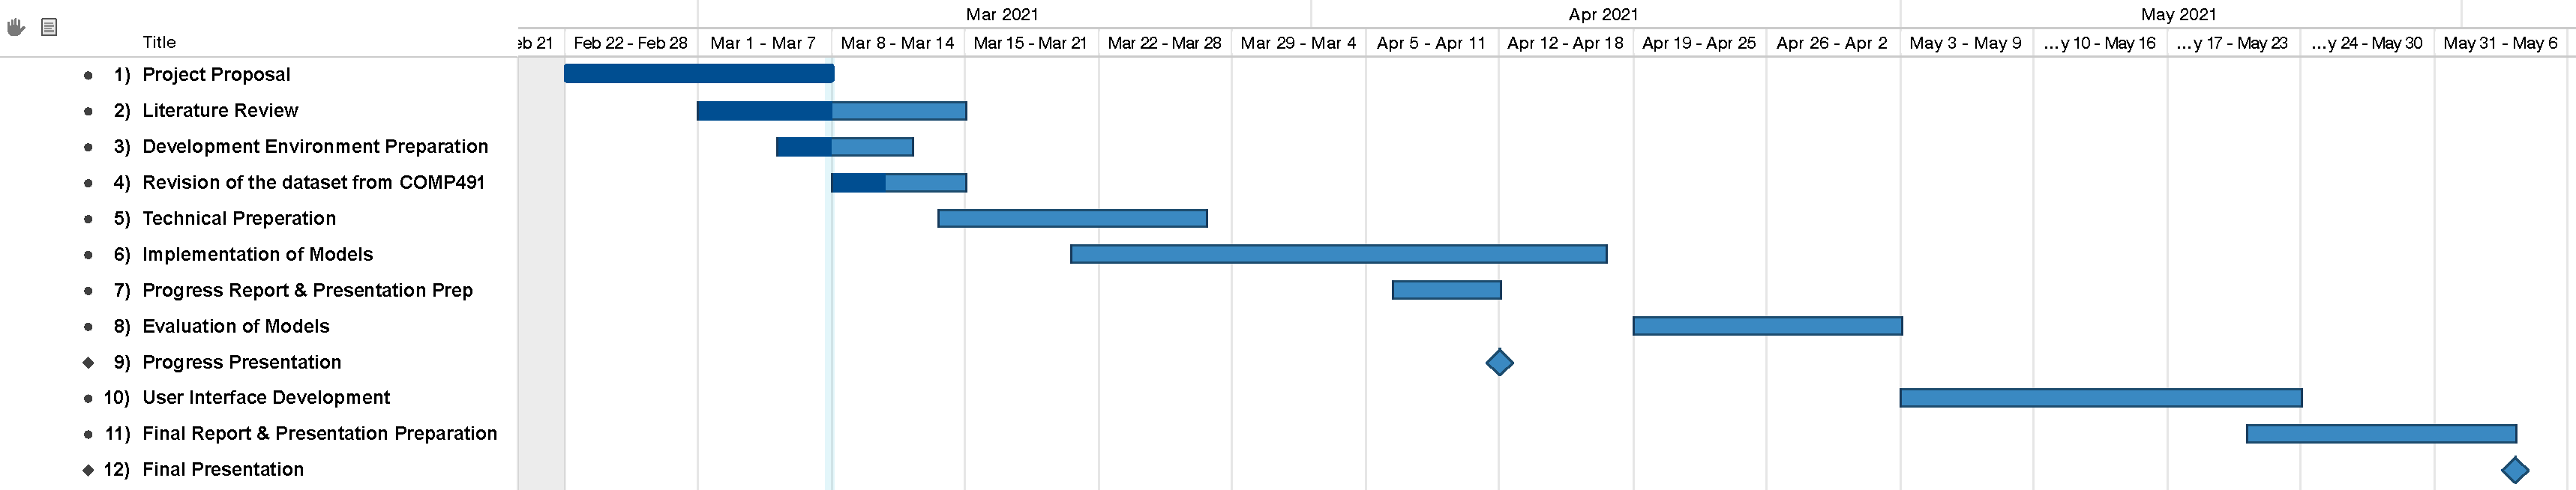
\includegraphics[width=0.95\textwidth]{../assets/gantt/gantt-chart.pdf}
		\caption{Gantt chart of the project}
	\end{figure}

	
	\section{Project Team and Authority Information}
	\begin{table}[H]
		\caption{Project team and authority information}
		\begin{tabularx}{\textwidth}{|>{\columncolor[RGB]{215,229,244}\hsize=0.33\hsize}X|
				>{\hsize=.67\hsize}X|} 	
			
			\hline
			\textbf{Proposal Date} & 08/03/2021 \\ \hline
			\textbf{Academic Term of Project Delivery} & 2020-2021, Spring \\ \hline
			\textbf{Project Team Members} & Alp Gokcek, \#041701014, Computer Engineering \newline Erdal Sidal Dogan, \#041701076, Computer Engineering  \\ \hline
			\textbf{Advisor(s)} & Seniz Demir \\ \hline
		\end{tabularx}
	\end{table}
\end{document}